\chapter{ACHIEVED RESULT}
\label{ch:chap3}
In this part, we will show the progress of system requirement specification and analysis, system design, implementation, testing and evaluation.
% Testing script is one of the core of testing framework.
% A testing script can be called a test case.
% This chapter describes the components that make up a testing script. At the end of chapter, there are some examples of testing scripts I use for experiments in Chapter \ref{ch:experiments}.

\section{System analysis and design}
\subsection{Requirement specification}
	\subsubsection{User requirement}
	Two types of actor in our system are user and administrator. Actor user is passenger who use mobile client application, actor admin is one who maintain database, manage buses information, approve user's requests. After analyzing the user need, we have the following user requirement table
	\begin{center}
		\begin{longtable}{|p{1cm}|p{1.5cm}|p{2.5cm}|>{\raggedright\arraybackslash}p{5cm}|p{2cm}|} 
			\hline
			\bfseries ID & \bfseries User type & \bfseries Action & \bfseries Description & \bfseries Note \\ 
			\hline\hline
			1 & User & Bus route look up & - User can look up for buses information such as price, operation time, go route and return route in map \newline
			- Bus station look up: bus stations which bus route goes through \newline
			- Nearby bus stations and bus route & \\ 
			\hline
			2 & User & Navigate by bus & - Allow navigate between 2 points in bus map \newline
			- Multiple criteria: least bus changes, shortest path, shortest walking  & \\ 
			\hline
			3 & User & Report out dated buses and create new bus route & - Allow user to report out dated buses and create new bus route  & \\ 
			\hline
			4 & User & Review reports and buses created & - Allow Review reports and buses created  & \\ 
			\hline
			5 & User Admin & Review user reports and buses created & - Admin can review reports and buses created from user & \\ 
			\hline
			6 & User Admin & Edit or Create bus information & - Admin can edit or add new buses information, bus stations & \\ 
			\hline
			\caption{User requirements}	
			\label{table:user_requirements} 
		\end{longtable}
	\end{center}

	\subsubsection{System requirement}

	\begin{center}
		\begin{longtable}{|p{1cm}|p{1.5cm}|p{2.5cm}|>{\raggedright\arraybackslash}p{5cm}|p{2cm}|} 
			\hline
			\bfseries ID & \bfseries Type & \bfseries Action & \bfseries Description & \bfseries Note \\ 
			\hline\hline
			1 &  & List all available provinces and buses route & Show a list of all available provinces and buses route in these province & \\ 
			\hline
			2 &  & Get user's current location and show related information & Get user's current location and show related information such as nearby bus stations and buss route & \\ 
			\hline
			3 &  & Information must be presented clearly and detailed & a route details will have to provide full information such as uptime, time spacing between each other, fare, go route and return route & \\ 
			\hline
			4 &  & Represent bus route by map & Represent bus route by map  & \\ 
			\hline
			5 &  & Review user reports and buses created & - Admin can review reports and buses created from user & \\ 
			\hline
			6 &  & Provide bus station information & For each bus route, show all bus station that that route go through and show name, buses that go through it & \\ 
			\hline
			7 &  & Input in Navigate function & Allow user to input both text and exactly location in map for start point and end point. Text input will not be distinguished capitalize. Location input can be current location or any other  & \\ 
			
			\hline
			8 &  & Show navigate result & - Show result in multiple criteria \newline - Result must be shown in map (clearly and friendly interface) \newline - Show guide in text & \\ 
			\hline
			9 &  & Allow choose bus route to report & - Show result in multiple criteria \newline - Result must be shown in map (clearly and friendly interface) \newline - Show guide in text & \\ 
			\hline
			10 &  & Allow choose type to report & - Show result in multiple criteria \newline - Result must be shown in map (clearly and friendly interface) \newline - Show guide in text & \\ 
			\hline
			11 &  & ... & ... & \\ 
			\hline

			\caption{System requirements}
			\label{table:system_requirements} 
		\end{longtable}
	\end{center}

\subsection{Requirement analysis}
	\subsubsection{Use cases diagram}
		\begin{figure}[H]
			\centering
			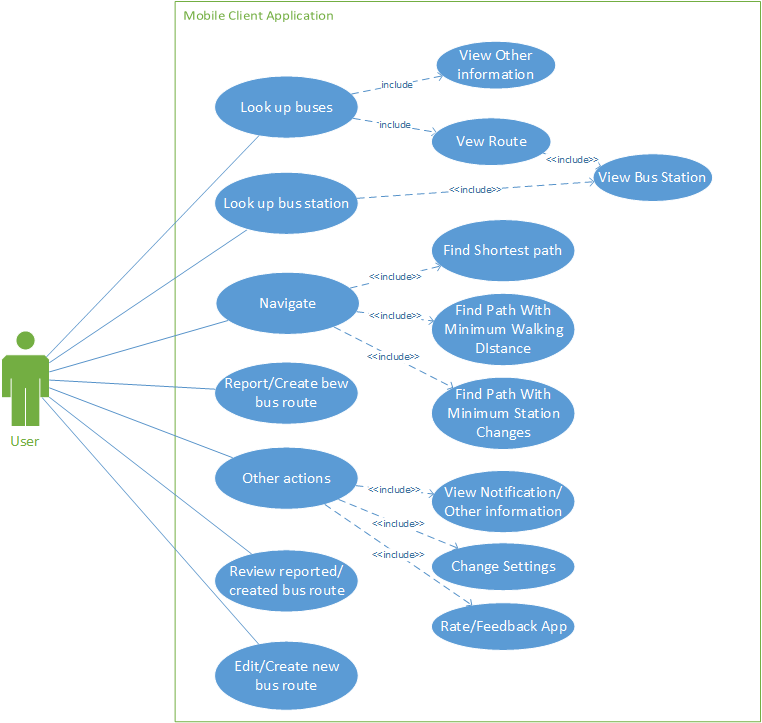
\includegraphics[scale=4]{Chapters/Fig/user-use-case.png}
			\caption{User use case diagram}
			\label{fig:user_use_case}
		\end{figure}

		\begin{figure}[H]
			\centering
			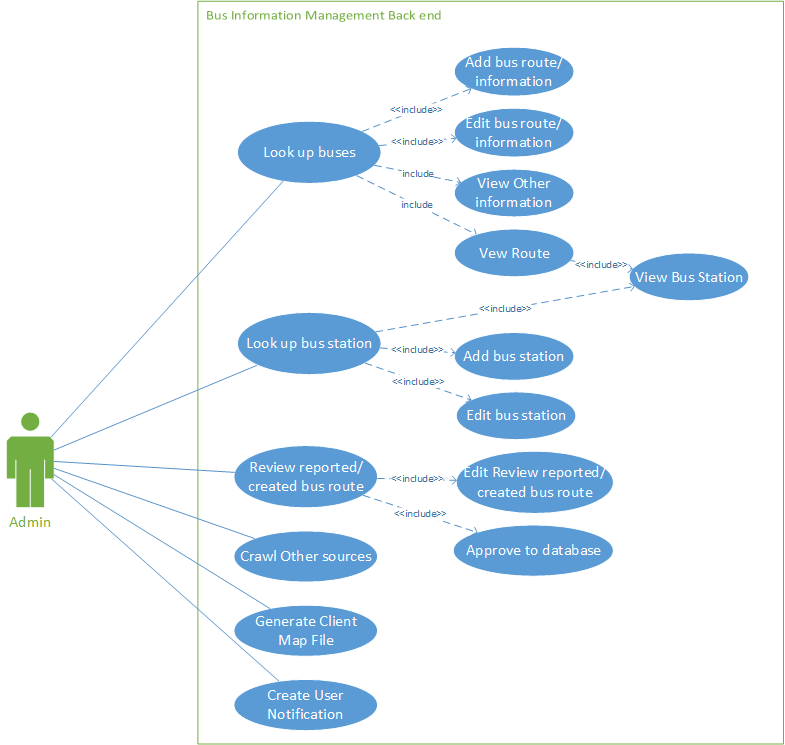
\includegraphics[scale=4]{Chapters/Fig/admin-use-case.png}
			\caption{Admin use case diagram}
			\label{fig:admin_use_case}
		\end{figure}

	\subsubsection{Use cases specification}
		\begin{center}
			\begin{longtable}{|p{3cm}||p{3cm}|p{3cm}|p{4cm}|} 
				\hline
				\bfseries UC Code & UC001 & \bfseries UC Name & Look up buses \\ 
				\hline
				\bfseries Actor & \multicolumn{3}{|c|}{User} \\
				\hline
				\bfseries Pre-condition & \multicolumn{3}{|c|}{None} \\
				\hline
				\bfseries Main Success Scenario (Flow of event) & \multicolumn{3}{|c|}{...} \\
				\hline
				\bfseries Extension Scenarios (Alternative flows) & \multicolumn{3}{|c|}{...} \\
				\hline
			\end{longtable}

			\begin{longtable}{|p{3cm}||p{3cm}|p{3cm}|p{4cm}|} 
				\hline
				\bfseries UC Code & UC002 & \bfseries UC Name & Look up bus stations \\ 
				\hline
				\bfseries Actor & \multicolumn{3}{|c|}{User} \\
				\hline
				\bfseries Pre-condition & \multicolumn{3}{|c|}{None} \\
				\hline
				\bfseries Main Success Scenario (Flow of event) & \multicolumn{3}{|c|}{...} \\
				\hline
				\bfseries Extension Scenarios (Alternative flows) & \multicolumn{3}{|c|}{...} \\
				\hline
			\end{longtable}

			\begin{longtable}{|p{3cm}||p{3cm}|p{3cm}|p{4cm}|} 
				\hline
				\bfseries UC Code & UC003 & \bfseries UC Name & Navigate \\ 
				\hline
				\bfseries Actor & \multicolumn{3}{|c|}{User} \\
				\hline
				\bfseries Pre-condition & \multicolumn{3}{|c|}{None} \\
				\hline
				\bfseries Main Success Scenario (Flow of event) & \multicolumn{3}{|c|}{...} \\
				\hline
				\bfseries Extension Scenarios (Alternative flows) & \multicolumn{3}{|c|}{...} \\
				\hline
				\caption{Use cases specifications} 
				\label{table:use_cases_specifications} 
			\end{longtable}

		\end{center}

\subsection{System design}
	\subsubsection{System Architecture Overview}
		\paragraph{System scenario}
			\begin{figure}[H]
				\centering
				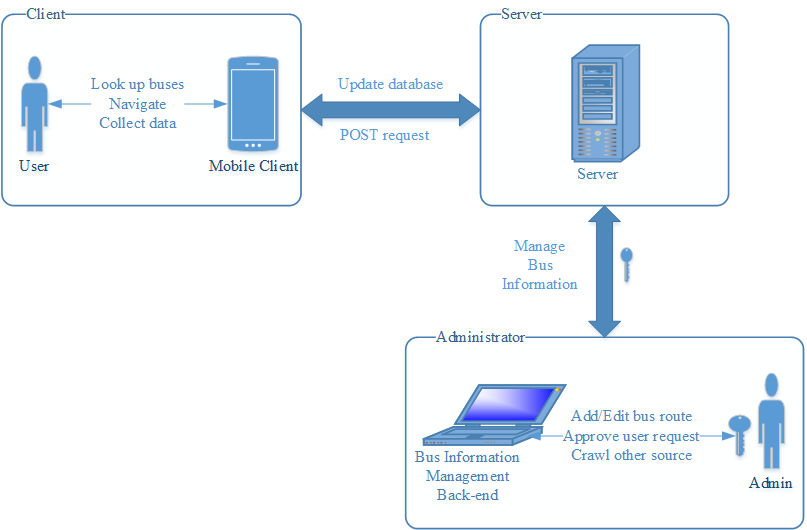
\includegraphics[scale=4.0]{Chapters/Fig/system-scenario.png}
				\caption{System scenario}
				\label{fig:system-scenario}
			\end{figure}
			The figure above present the system scenario, the scenario included:
			\begin{itemize}
				\item \textbf{User}: also called passenger, are users who use mobile application to look up for buses, navigate and collect data.
				\item \textbf{Mobile application)}: a mobile application client with basic functions allows user to look-up and navigate, also collect data functions to report outdated buses route and build new buses route which is not exist.
				\item \textbf{Server}: include database and a web service to interact with mobile client application, which provide APIs that allow client to check update database, get new notification, and post collected data.
				\item \textbf{Admin}: are people who manage bus information system, have permissions to add/edit buses route, review and approve user request, create notification to user.
				\item \textbf{Management Application}: for admin manage buses route information, process collected data, crawl other sources, generate client map file and create new notification to users.
			\end{itemize}

		\paragraph{System modules}	
			From the scenario, we divide it into three components:
			\newpage
			\begin{landscape}
			\begin{figure}[H]
				\centering
				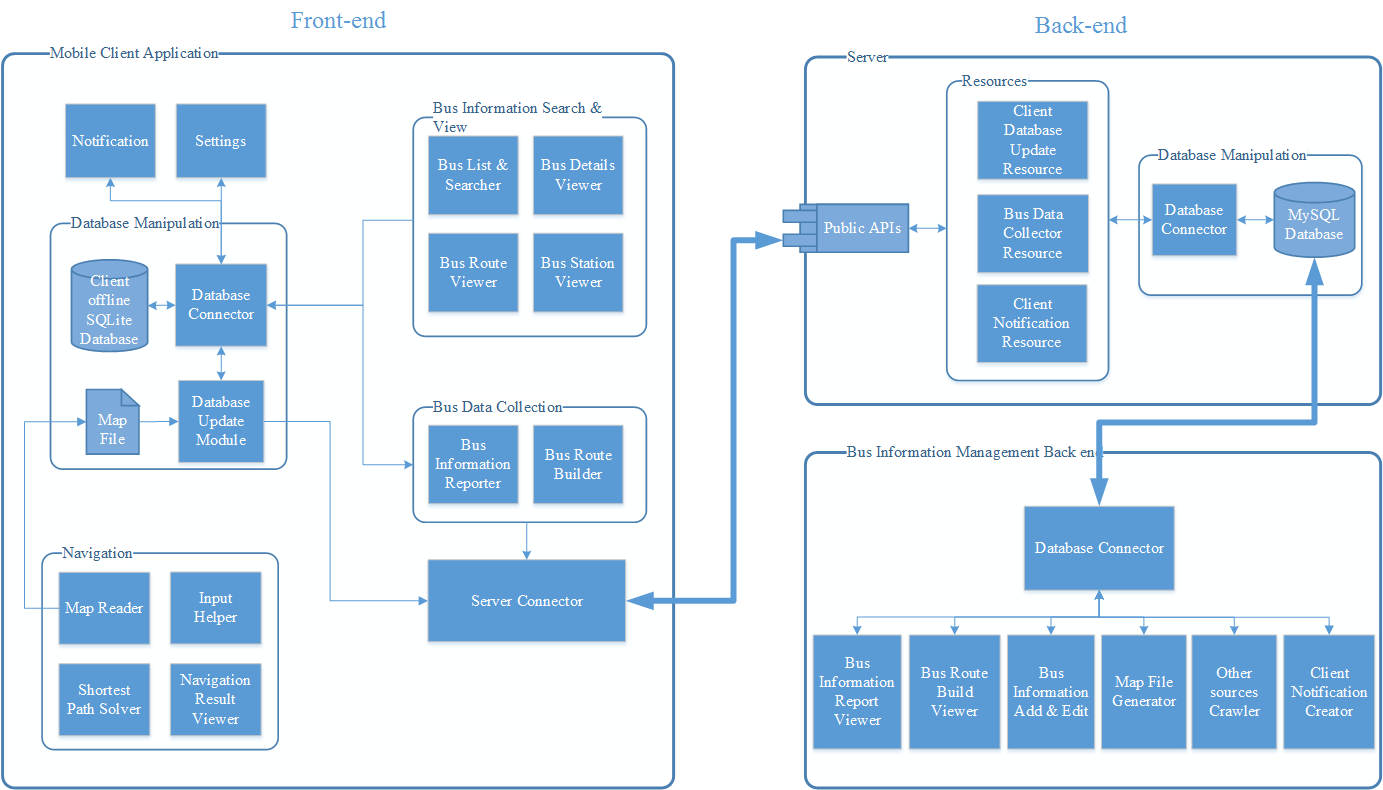
\includegraphics[scale=4.0]{Chapters/Fig/System-architecture-overview-details.png}
				\caption{System architecture overview}
				\label{fig:system-architecture-overview}
			\end{figure}
			\end{landscape}
			\newpage
		
		Each module has its specific mission:
		\begin{itemize}
			\item \textbf{Mobile Client application}:
				\begin{itemize}
					\item[--] \textbf{Buses list and searcher}: list all bus in each province, provide search function to help user search and select a bus easily.
					\item[--] \textbf{Buses details viewer}: show all details of a bus like operation time, frequency, fare, route in text...
					\item[--] \textbf{Buses route viewer}: show bus route in map with each through station
					\item[--] \textbf{Buses station viewer}: show all details of a bus station, its name, location and all buses that through it.
					\item[--] \textbf{Buses information reporter}: a module that help user to report incorrect bus information, edit bus information, route and then post data to server.
					\item[--] \textbf{Buses route builder}: a module that allow user to create a new bus which is not exist in current database. User can add bus's name, information, and route and then post data to server.
					\item[--] \textbf{Server connector}: a module that contains server's information, server's APIs, provide methods that help all other modules to interact with server.
					\item[--] \textbf{SQLite database and database connector}: store all data in sqlite file, provide methods that help all other modules to manipulate with database.
					\item[--] \textbf{Database Update module}: a module that keeps client's database always up-to-date with server's database.
					\item[--] \textbf{Map file and Map Reader}: map file is generated by back-end, corresponding to bus data changing, used for navigate algorithm.
					\item[--] \textbf{Input helper}: in navigation, help user to input start location and end location easily, user can input text like street name, station's name, or geo-location.
					\item[--] \textbf{Shortest path solver}: an algorithm module for finding suitable path based on each criteria (shortest path, path with minimum station changes, path with minimum walking distance)
					\item[--] \textbf{Navigation result viewer}: show navigate result in map with detailed guide for user
					\item[--] \textbf{Notification}: get notification from server and show to user.
					\item[--] \textbf{Settings}: allow user to change some settings such as minimum walking distance from each station, application theme...
				\end{itemize}
			\item \textbf{Server}: 
				\begin{itemize}
					\item[--] \textbf{MySQL database and database connector}: store all data in MySQL, provide methods that help all other modules to manipulate with database.
					\item[--] \textbf{Resources}: each resource provide a public API that allow client to GET or POST data. Details of each resource will be show on section \ref{sssec:server_design}
				\end{itemize}
			\item \textbf{Bus Information Management Back-end}: 
				\begin{itemize}
					\item[--] \textbf{Bus information report viewer}: list all user report request, show details of each request, allow admin to edit and approve that request.
					\item[--] \textbf{Bus route build viewer}: list all user created bus request, show details of each request, allow admin to edit and approve that request.
					\item[--] \textbf{Bus information add \& edit}: show all buses, allow admin to add and edit bus information.
					\item[--] \textbf{Other sources crawler}: provide methods that help admin to crawl other exist source.
					\item[--] \textbf{Map file generator}: generate client map file, upload to server.
					\item[--] \textbf{Client notification creator}: help admin to notify to user about updated buses, news...
				\end{itemize}
		\end{itemize}
	\subsubsection{Database Designing}
		The database designed quite simply to store all bus information, bus station information, provinces, user request, notification and current database version.
		\paragraph{Modeling data} 	
			From above requirement analysis, we model data using ER diagram as below:
			\begin{figure}[H]
				\centering
				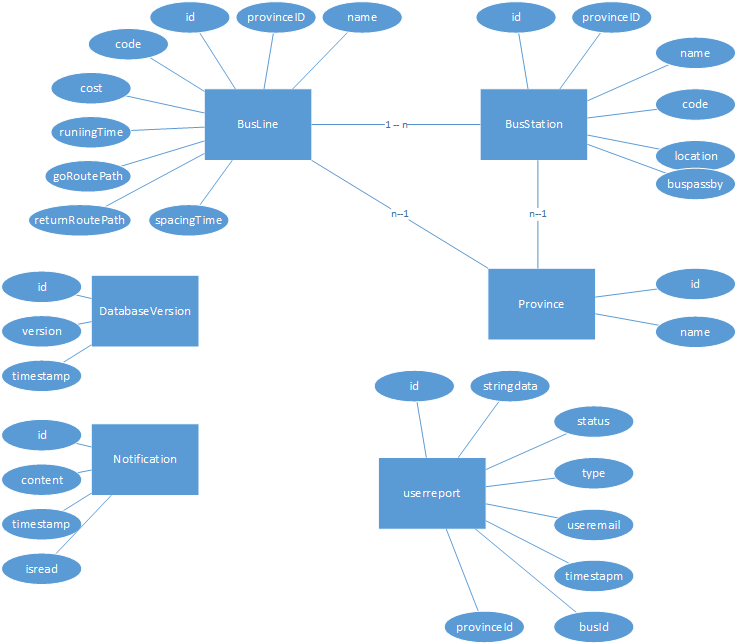
\includegraphics[scale=5]{Chapters/Fig/ER-model.png}
				\caption{ER Model}
				\label{fig:ER-model}
			\end{figure}
		\paragraph{Logical Data schema} 
			From above data modeling, we designed a database with these tables:
			\begin{figure}[H]
				\centering
				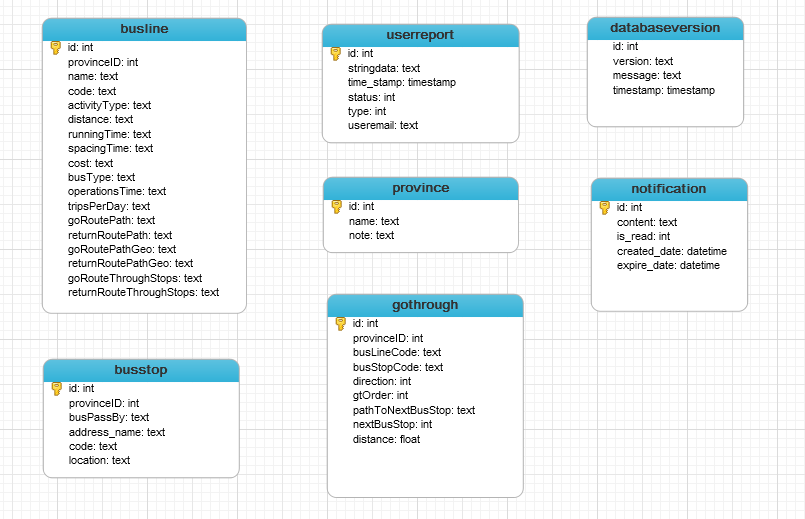
\includegraphics[scale=0.7]{Chapters/Fig/database-design.png}
				\caption{Database design}
				\label{fig:database-design}
			\end{figure}

			\begin{itemize}
				\item{Table busline}: store bus information, route: 
					\begin{center}
						\begin{longtable}{|p{4cm}|p{2cm}|p{3cm}|>{\raggedright\arraybackslash}p{5cm}|} 
							\hline
							\bfseries Name & \bfseries Type & \bfseries Constraint & \bfseries Comment\\ [0.5ex] 
							\hline\hline
							id & Int & PK & ID of this bus \\
							\hline
							provinceId & Int & FK(province.id) & ID of province that this bus belong to \\
							\hline
							activityType, distance, runningTime, spacingTime, cost, busType, operationsTime, tripsPerDay, goRoutePath, returnRoutePath, goRoutePathGeo, returnRoutePathGeo & Text & & Details of this bus \\
							\hline
							goRouteThroughStops, returnRouteThroughStops & Text & & List of bus station id, present each bus station which this bus pass through. Eg: 1 3 4 6 8 means this bus pass through bus station id 1,3,4,6 and 8. \\
							\hline
							\caption{Bus Line table details}	
							\label{table:busline_table} 
						\end{longtable}
					\end{center}
				\item{Table province}: store all available province
					\begin{center}
						\begin{longtable}{|p{4cm}|p{2cm}|p{3cm}|>{\raggedright\arraybackslash}p{5cm}|} 
							\hline
							\bfseries Name & \bfseries Type & \bfseries Constraint & \bfseries Comment\\ [0.5ex] 
							\hline\hline
							id & Int & PK & ID of this province \\
							\hline
							name & Int & & ID of province that this bus belong to \\
							\hline
							note & Text & & Reverse for future \\
							\hline
							\caption{Province table details}	
							\label{table:province_table} 
						\end{longtable}
					\end{center}
				\item{Table busstation}: store bus station details: 
					\begin{center}
						\begin{longtable}{|p{4cm}|p{2cm}|p{3cm}|>{\raggedright\arraybackslash}p{5cm}|} 
							\hline
							\bfseries Name & \bfseries Type & \bfseries Constraint & \bfseries Comment\\ [0.5ex] 
							\hline\hline
							id & Int & PK & ID of this bus station \\
							\hline
							provinceId & Int & FK(province.id) & ID of province which this bus belong to \\
							\hline
							buspassby & Text & & store id of bus which this bus station belong to \\
							\hline
							addressname, code, location & Text & & Details of this bus station \\
							\hline
							\caption{Bus station table details}	
							\label{table:busstation_table} 
						\end{longtable}
					\end{center}
				\item{Table databaseversion}: store versions of database, change log. 
					\begin{center}
						\begin{longtable}{|p{4cm}|p{2cm}|p{3cm}|>{\raggedright\arraybackslash}p{5cm}|} 
							\hline
							\bfseries Name & \bfseries Type & \bfseries Constraint & \bfseries Comment\\ [0.5ex] 
							\hline\hline
							id & Int & PK & ID of this version \\
							\hline
							version & Int & & Version in text. Eg: 1.0.0.2\\
							\hline
							message & Text & & Changes, detail about this version. \\
							\hline
							timestamp & Timestamp & & store time stamp when new database version is created \\
							\hline
							\caption{Database Version table details}	
							\label{table:databaseversion_table} 
						\end{longtable}
					\end{center}
				\item{Table notification}: store notification to notify users
					\begin{center}
						\begin{longtable}{|p{4cm}|p{2cm}|p{3cm}|>{\raggedright\arraybackslash}p{5cm}|} 
							\hline
							\bfseries Name & \bfseries Type & \bfseries Constraint & \bfseries Comment\\ [0.5ex] 
							\hline\hline
							id & Int & PK & ID of this bus \\
							\hline
							content & Text & FK(province.id) & ID of province that this bus belong to \\
							\hline
							createddate, expiredate & Timestamp & & Created and Expire time of this notification \\
							\hline
							\caption{Notification table details}	
							\label{table:notification_table} 
						\end{longtable}
					\end{center}
				\item{Table userreport}: store user request about incorrect bus information and add new non-exist bus
					\begin{center}
						\begin{longtable}{|p{4cm}|p{2cm}|p{3cm}|>{\raggedright\arraybackslash}p{5cm}|} 
							\hline
							\bfseries Name & \bfseries Type & \bfseries Constraint & \bfseries Comment\\ [0.5ex] 
							\hline\hline
							id & Int & PK & ID of this bus \\
							\hline
							stringdata & Text & & data of request in JSON format \\
							\hline
							status & Int & & Status of this request. Eg: Approved or not \\
							\hline
							type & Int & & Type of this request. Eg: report incorrect route request or add new bus request \\
							\hline
							useremail & Text & & Email of user who sent this request \\
							\hline
							\caption{User report table details}	
							\label{table:userreport_table} 
						\end{longtable}
					\end{center}
			\end{itemize}
	\subsubsection{Server (Web service) Design} \label{sssec:server_design}
		Missions of web service is allow users to get latest data, accept user's post requests, which are report outdated route request and build new bus route request, also is a point to interact between admin and users, help admin to notify users about database update, changes...
		From these missions, we specialize into web service's APIs as below:
		\paragraph{APIs design}
			\begin{center}
			\begin{longtable}{|p{1cm}|p{2cm}|p{5cm}|p{6cm}|} 
				\hline
				\bfseries No & \bfseries Type & \bfseries Resource Name & \bfseries Mission \\ 
				\hline
				\hline
				1 & GET & SqliteDbDownloadResource & Allow client to check latest version of database and provide link to download sqlite version \\
				\hline
				2 & POST & UserReportResource & Accept POST request from client, allow client to report outdated bus route and build new bus route which is not exist \\
				\hline
				3 & GET & ClientNotificationResource & Notify all users about database update, changes... \\
				\hline
				\caption{RESTfull Web service API Design} 
				\label{table:RESTfull_Web_service_API_Design} 
			\end{longtable}
			\end{center}
		\paragraph{Security}
		Since our web service is stateless and no user authentication or roles requires, there are two things we need to secure is SQL injection in post requests from users and DDOS attack, other types such as protect HTTP method, validate incoming content-types, resources URL check will be handle by build-in Java framework. Details will be provide in \'System development\' section.
		
	\subsubsection{Client Design}
		\paragraph{Architecture design}
			\begin{figure}[H]
				\centering
				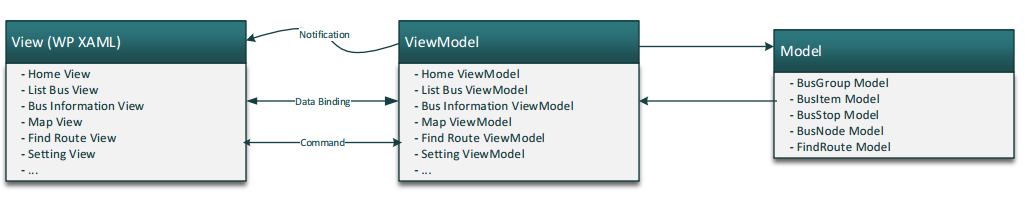
\includegraphics[scale=0.5]{Chapters/Fig/client-architecture-design.png}
				\caption{client-architecture-design}
				\label{fig:architecture-of-webservice}
			\end{figure}
		\paragraph{Modeling \& UML}
			\begin{figure}[H]
				\centering
				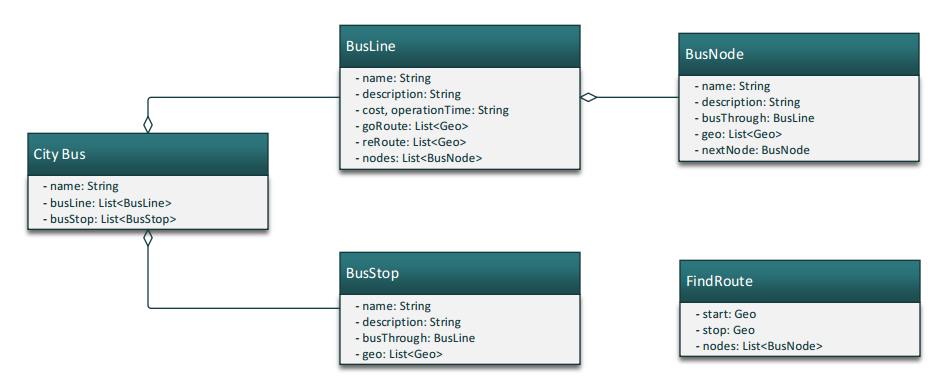
\includegraphics[scale=0.6]{Chapters/Fig/client-model-classes.png}
				\caption{client-model-classes}
				\label{fig:architecture-of-webservice}
			\end{figure}
			\begin{figure}[H]
				\centering
				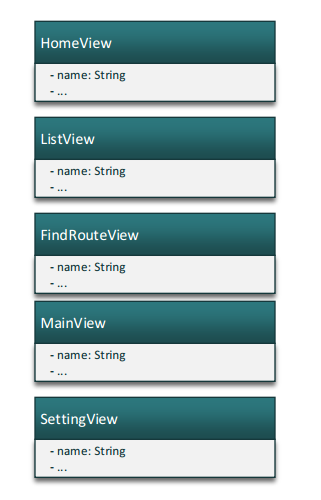
\includegraphics[scale=0.7]{Chapters/Fig/client-view-classes.png}
				\caption{client-view-classes}
				\label{fig:architecture-of-webservice}
			\end{figure}
			\begin{figure}[H]
				\centering
				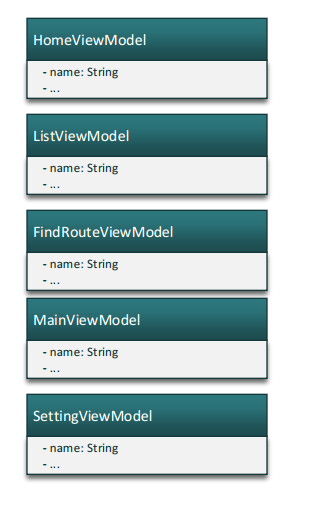
\includegraphics[scale=0.7]{Chapters/Fig/client-view-model-classes.png}
				\caption{client-view-model-classes}
				\label{fig:architecture-of-webservice}
			\end{figure}
		\paragraph{Sequence diagrams}
			\begin{itemize}
				\item{Bus Information Search \& View}
					\begin{figure}[H]
					\centering
					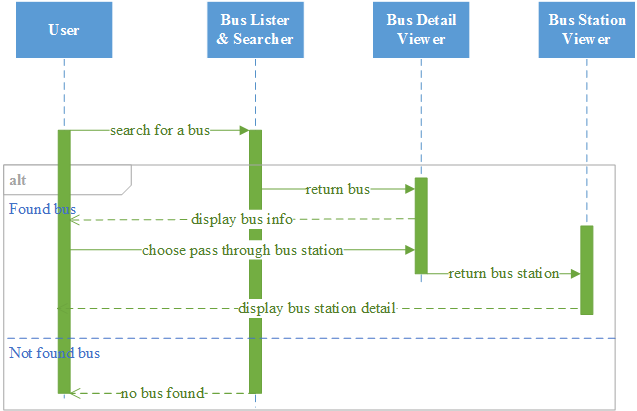
\includegraphics[scale=5]{Chapters/Fig/bus-search-and-view-sd.png}
					\caption{Bus Information Search \& View Sequence Diagram}
					\label{fig:bus_view_sd}
					\end{figure}
				\item{Navigation}
					\begin{figure}[H]
					\centering
					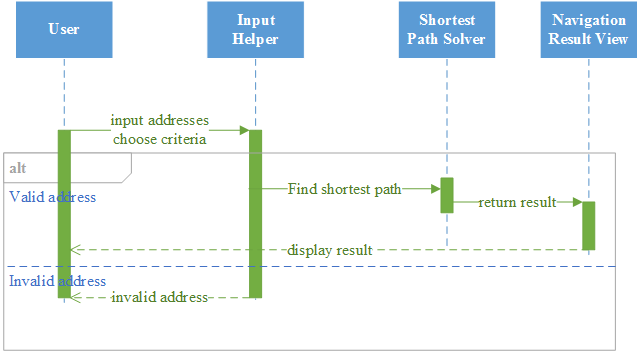
\includegraphics[scale=5]{Chapters/Fig/navigate-sd.png}
					\caption{Navigation Sequence Diagram}
					\label{fig:navigate_sd}
					\end{figure}
				\item{Bus Information Report}
					\begin{figure}[H]
					\centering
					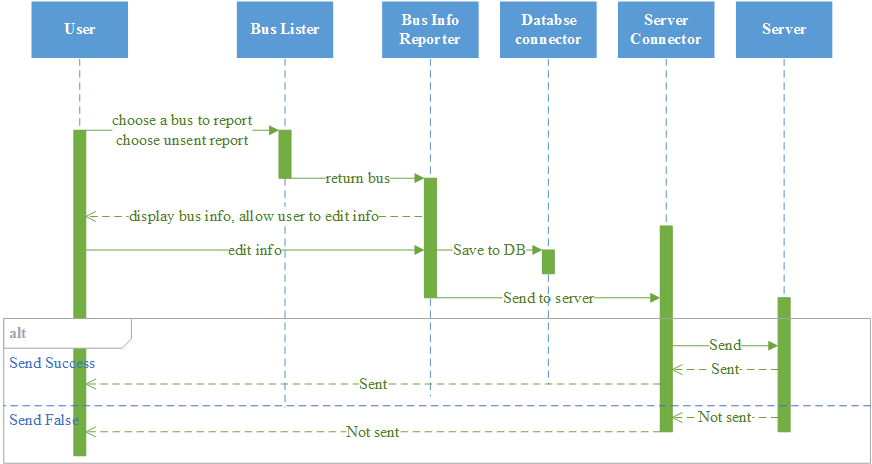
\includegraphics[scale=4]{Chapters/Fig/bus-report-sd.png}
					\caption{Bus Information Report Sequence Diagram}
					\label{fig:report_sd}
					\end{figure}
				\item{Bus Route Build}
					\begin{figure}[H]
					\centering
					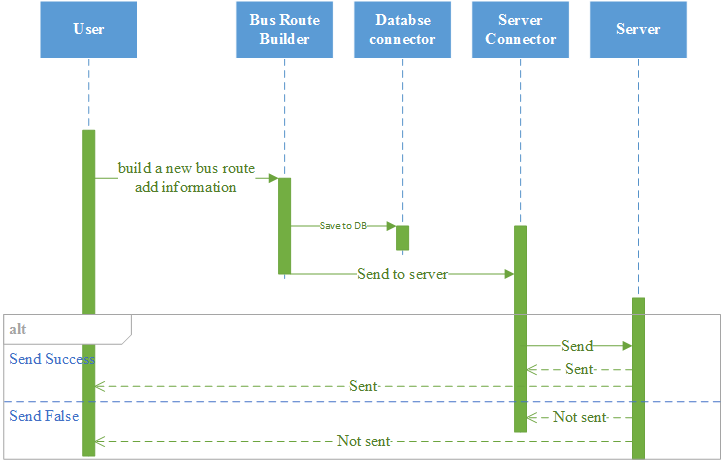
\includegraphics[scale=5]{Chapters/Fig/build-route-sd.png}
					\caption{Bus Route Build Sequence Diagram}
					\label{fig:build_route_sd}
					\end{figure}
			\end{itemize}
	\subsubsection{Client Mobile Application User Interface Design}
		\begin{figure}[H]
			\centering
			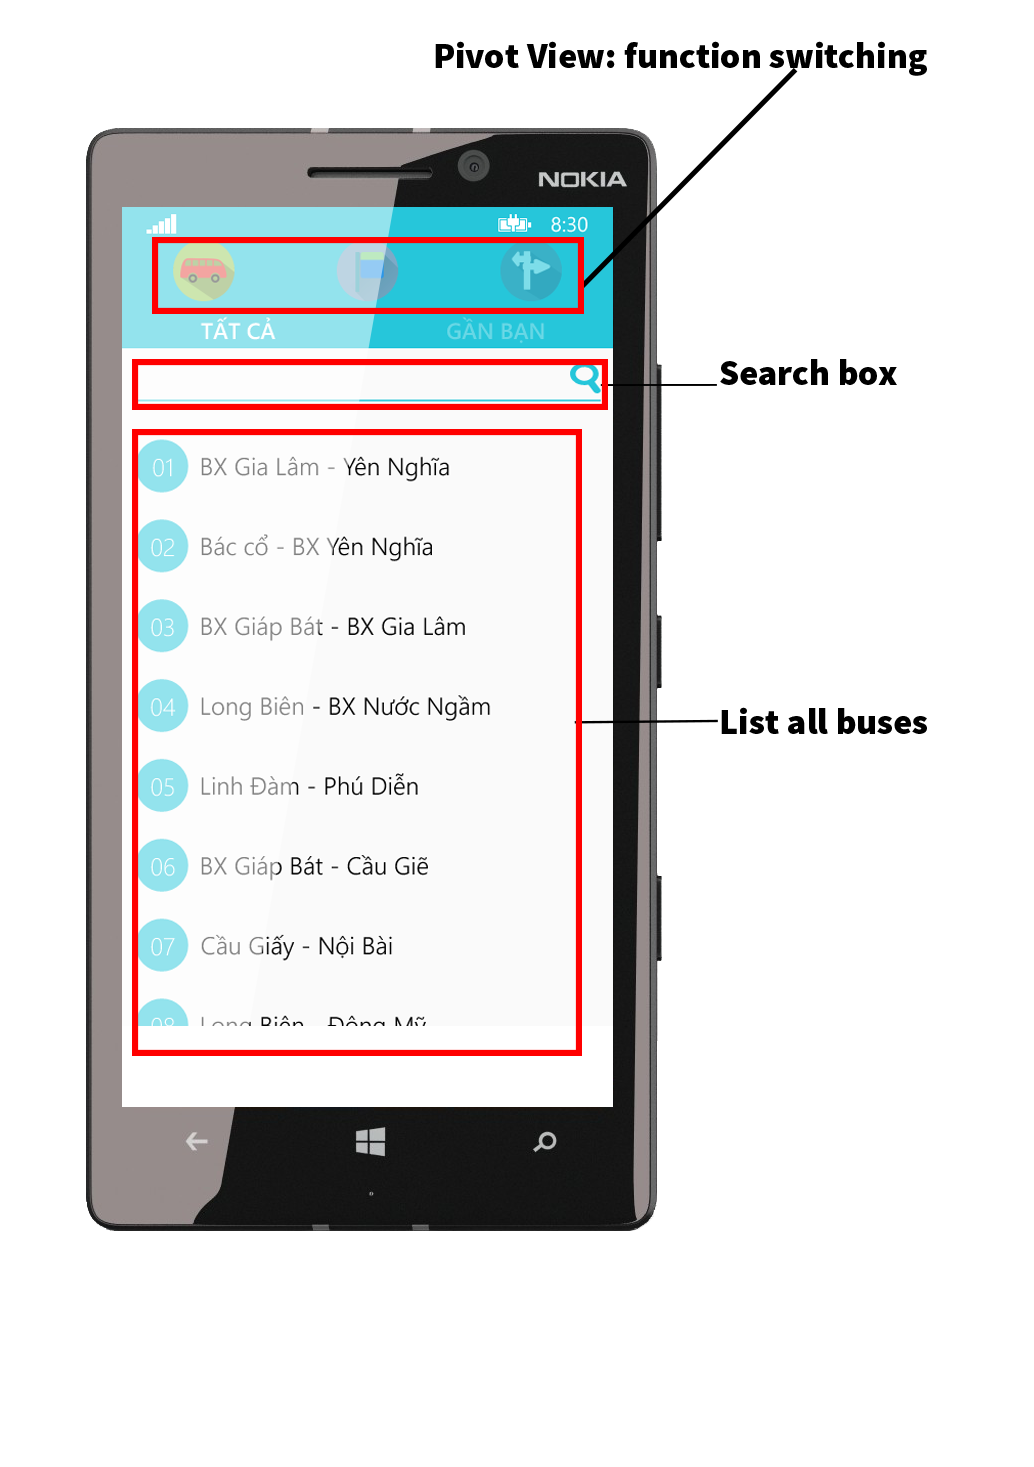
\includegraphics[scale=0.4]{Chapters/Fig/MainPivotView_inPhone.png}
			\caption{Main pivot view}
			\label{fig:architecture-of-webservice}
		\end{figure}
	\subsubsection{Management Application Design}


\section{System development}
\subsection{Development environment}
	\begin{itemize}
		\item{Mobile Client Application development environment}
		\begin{itemize}
			\item [--]{Operating System}: Microsoft Windows 10
			\item [--]{IDE}: Visual Studio 2015
			\item [--]{Virtual Machine}: Windows Phone 8.1 Emulator
			\item [--]{Database}: SQLite
			\item [--]{Source code control}: Git
			\item [--]{Programming Language}: C\#
		\end{itemize}
		\item{Server development environment}
		\begin{itemize}
			\item [--]{Operating System}: Microsoft Windows 10
			\item [--]{IDE}: Netbean 7
			\item [--]{Web server}: Apache Tomcat 6
			\item [--]{Database}: MySQL
			\item [--]{Source code control}: Git
			\item [--]{Programming Language}: Java
		\end{itemize}
		\item{Bus Information Management Back end development environment}
		\begin{itemize}
			\item [--]{Operating System}: Microsoft Windows 10
			\item [--]{IDE}: Visual Studio 2015
			\item [--]{Database}: MySQL
			\item [--]{Source code control}: Git
			\item [--]{Programming Language}: C\#
		\end{itemize}
	\end{itemize}
\subsection{Deployment environment}
	\begin{itemize}
		\item{Mobile Client Application deployment environment}
		\begin{itemize}
			\item [--]{Operating System}: Windows Phone 8.1
			\item [--]{Database}: SQLite
		\end{itemize}
		\item{Server deployment environment}
		\begin{itemize}
			\item [--]{Operating System}: CentOS 6
			\item [--]{Web server}: Apache Tomcat 6
			\item [--]{Database}: MySQL
		\end{itemize}
		\item{Bus Information Management Back end deployment environment}
		\begin{itemize}
			\item [--]{Operating System}: Microsoft Windows 10
			\item [--]{Database}: MySQL
		\end{itemize}
	\end{itemize}
\subsection{Implementation Web service}
	\subsection{Security}
		\indent First, SQL injection, for each incoming request, after verified data type, we're going to insert this request to database using SQL command:
			\begin{verbatim} String query = \"INSERT into userreport(stringdata, \end{verbatim}
			\begin{verbatim} time_stamp) values(?, NOW())\"; \end{verbatim}
		Next step is prepare about sql command statement
			\begin{verbatim} PreparedStatement stmt = dbConn.prepareStatement(query); \end{verbatim}
		Set data for above field in sql command, that field is denoted as '?':
			\begin{verbatim} stmt.setString(1, incomingData); \end{verbatim}
		Finally is execute command:
			\begin{verbatim} stmt.executeUpdate(); \end{verbatim}
		
		\indent Second, DDOS attack prevention, we put a HTTP cache in front of our API and put a small max-age header on any resource. Even having a max-age of 1 second will prevent your API from being hit more than once per second for that resource. Also, we limit the requests per source IP to sensible values, blocking IPs which exceed this burst limit more than a couple of times in a row.
\subsection{Implementation Mobile application}
\subsection{Implementation Management application}


\section{Testing and evaluations}
\subsection{Installation}
\subsection{Running the system}
\subsection{Result estimation}

% \section{Testing script components}
% \label{sec:script_comp}
% A testing script consists of one or more script actions. Each script action has following elements:
%     \begin{itemize}
% 		\item[--] \textbf{Source object}: element on the screen to be applied action on which is detected in Chapter \ref{ch:screen_recognize}
% 		\item[--] \textbf{Action}: what to do with source object, will be covered in Section \ref{sec:actions}.
% 		\item[--] \textbf{Execution time}: how long it takes to complete the action
% 		\item[--] \textbf{Expected object} (optional, depended on each action): after finishing action, what expected to be display on the screen
% 	\end{itemize}

% \subsection{Actions}
% \label{sec:actions}
% The robot is designed for physically contacting with the phone. It simulates human operations to perform testing process.
% There are 4 basic actions for robot to apply on mobile phone screen:
%     \begin{itemize}
% 		\item[--] \textbf{Click}: perform a quick single tap on screen
% 		\item[--] \textbf{Hold}: tap and keep pointer on the screen for a short time then release
% 		\item[--] \textbf{Drag}: tap on the screen, move pointer to a certain location then release
% 		\item[--] \textbf{Flick}: tap on the screen and quickly move pointer apart and release
% 	\end{itemize}

% \subsection{States of system}
%     \begin{figure}[H]
% 		\centering
% 		\includegraphics[scale=0.7]{Chapters/Fig/system_state.png}
% 		\caption{System state diagram}
% 		\label{fig:system_state}
% 	\end{figure}


% \subsection{System sequence diagram}
%     \begin{figure}[H]
% 		\centering
% 		\includegraphics[scale=0.75]{Chapters/Fig/sequence_diagram.png}
% 		\caption{System sequence diagram}
% 		\label{fig:sequence_diagram}
% 	\end{figure}

% \section{Testing script example}
% \label{sec:eg_script}
% \subsection{Simple click test}
% Flow diagram of script
% 	\begin{figure}[H]
% 		\centering
% 		\includegraphics[scale=0.55]{Chapters/Fig/click_test_diag.png}
% 		\caption{Simple Click Test flow diagram}
% 		\label{fig:click_test_diag}
% 	\end{figure}

% \subsection{Set alarm test}
% Flow diagram of script
% 	\begin{figure}[H]
% 		\centering
% 		\includegraphics[scale=0.55]{Chapters/Fig/alarm_test_diag.png}
% 		\caption{Set Alarm Test flow diagram}
% 		\label{fig:alarm_test_diag}
% 	\end{figure}
